\section{Game Design}

% Base on our pilot study results, we understand that if the cooperative game require High-Level Feature Communication, play it with non-common language player is really frustrating. According to GameFlow[1], games challenging should match the player’s skill level, If the challenges are greater than the skills, the result is anxiety and frustrating, if the challenges are less than the skills, the result is apathy and boring.

%Based on our pilot study results(see Table 2). We realize that if playing cooperative games requires high-level-feature communication, playing with different language players would feel deeply frustrated. According to GameFlow\cite{GD1}, game challenges should match the player's skill level. If the challenges are greater than the player's skills, the result of gameplay will be anxious and frustrating. But, by contrast, if the challenges are less than the player's skills, the result will be apathy and bored.

GameFlow\cite{GD1} discussed how game difficulty and players' skill levels affect whether players would perceive the experience as boring, fun, or frustrating. As shown Figure~\ref{fig:GD_F1}, when the difficulty is greater than the player's skills, the experience is frustrating. On the other hand, when the difficulty is less than the player's skills, the experience will be boring.


\begin{figure}[!b]
\centering
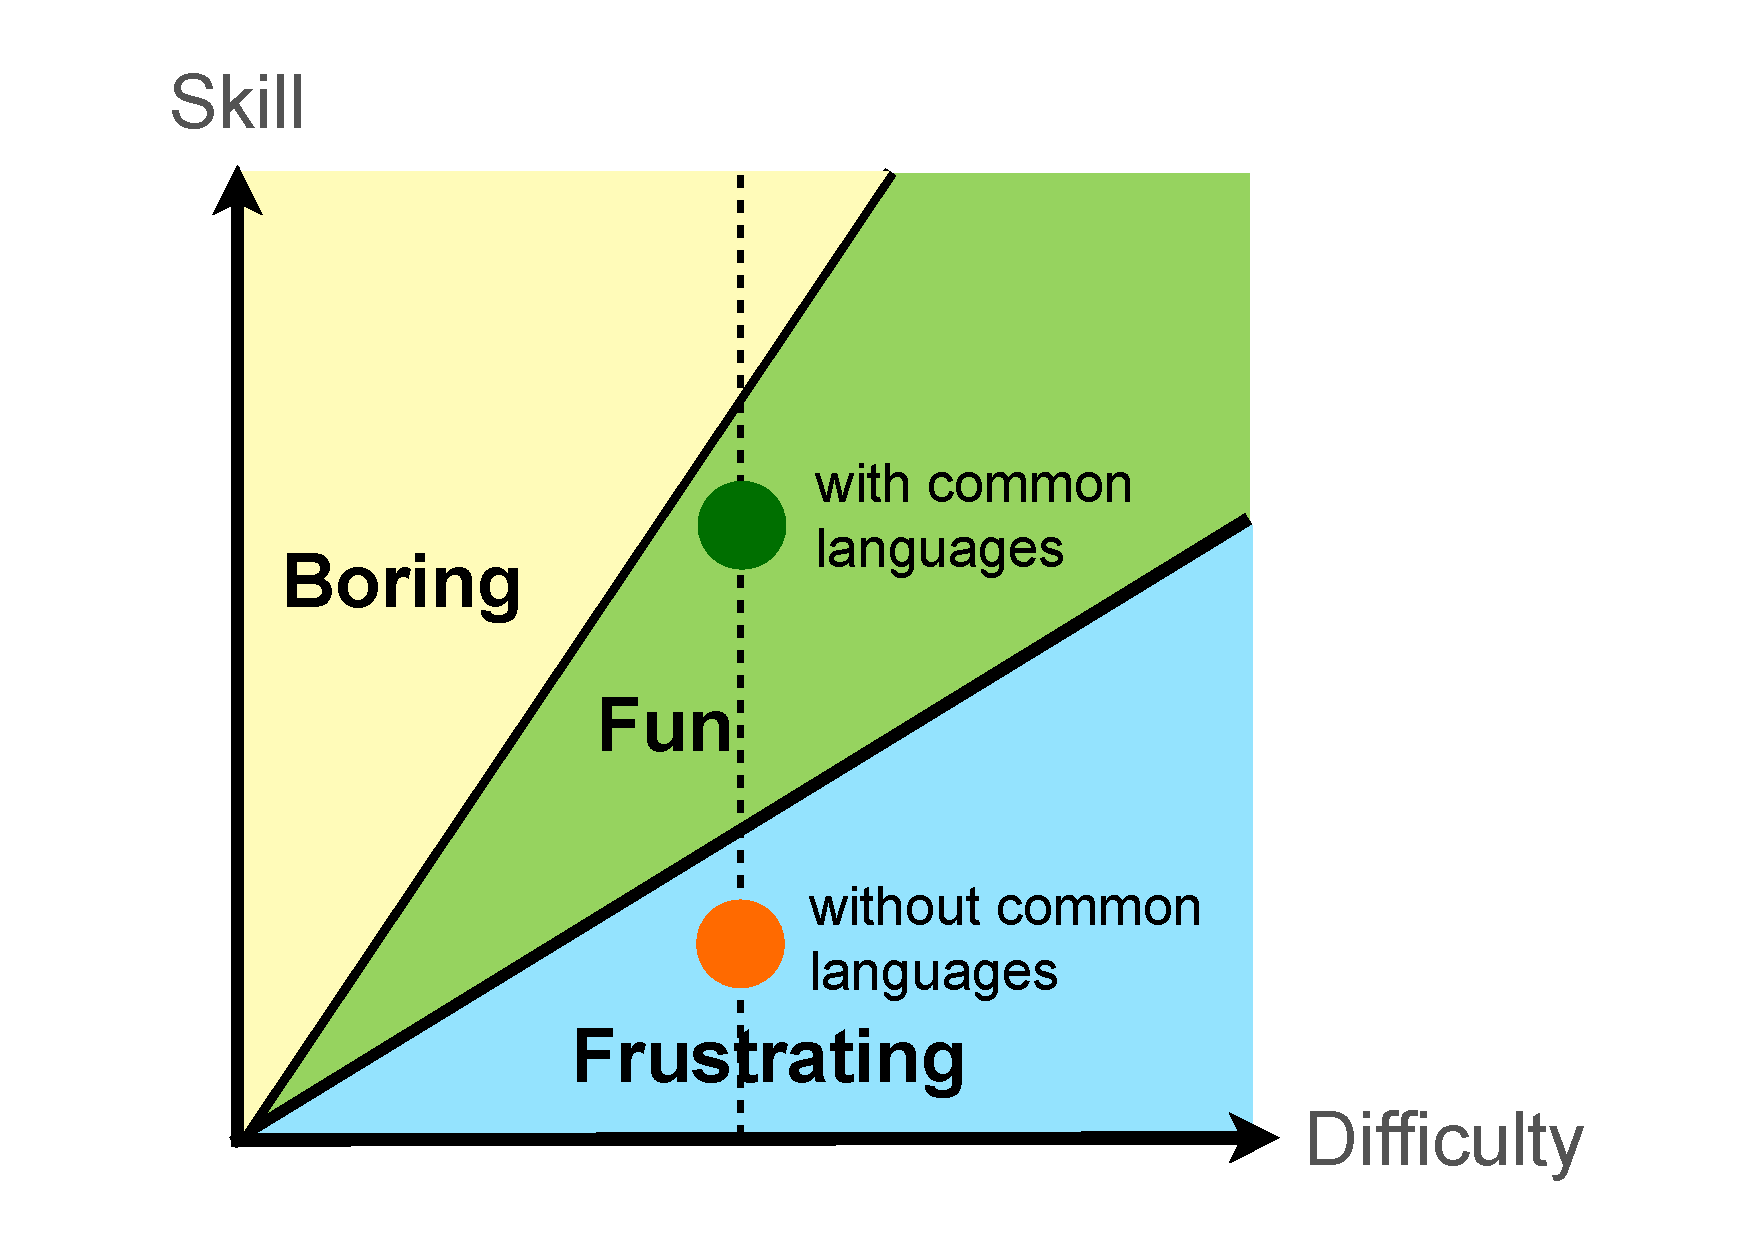
\includegraphics[width=0.9\columnwidth]{Figures/GD_F1.pdf}
\caption{Players cooperative skill levels are lower without a common language. Adding body language communication increases them, and may move the experience from being frustrating to fun.}
\label{fig:GD_F1}
\end{figure}

% According to our observation, play cooperative game with different language speaker will significantly decrease cooperative skills which is really important for most cooperative games and the game challenge become too hard for this situation and causing frustrating. The most easy way to solve this problem is to decrease the game challenge difficulty for non-common language players, but it is not practical for commercial games because the players with common language would feel boring with no difficulty.

Observation from our study indicated that playing a cooperative game with a partner that did not have a common language significantly decreased players' skill level. At a difficulty level that was designed to be fun for players with common languages, that difficulty level was too challenging for players that could not communicate through languages, which lead to a frustrating experience. 

One way to solve this problem is to decrease the game's difficulty. However, this method makes the experience boring for players that had common languages. By adding body language to the gameplay, players without common languages would be able to increase their skill level, and potentially move the experience from frustrating to fun (as shown in Figure~\ref{fig:GD_F1}).  



% \subsection{Body Language}

% % Human communication involves not only speech, but also a wide variety of gestures and body motions. Body language is the most effective means of communicating un-spoken emotions, a non-verbal way to impart your thoughts without verbalizing it. According to The 7\% Rule [1], communication is only 7 percent verbal and 93 percent non-verbal. The non-verbal component was made up of body language(55 percent) and tone of voice (38 percent).

% Consist of human communication, there is not only speech but also inclusive of various gestures and body motions. Body language, a non-verbal way to transmit your thoughts without verbalizing. According to The 7\% Rule\cite{GD2}, the influence of communication for verbal is only 7\% but is 93\% for non-verbal expression. And the non-varbal expression is made up of body language (55\%) and tones of voice (38\%).

% % Charades[2] is a word guessing game.In the form most played today, it is an acting game in which one player acts out a word or phrase, often by miming similar sounding words, and the other players guess the word or phrase. The idea is to use physical rather than verbal language to convey the meaning to another party.

% Charades\cite{GD3} is a word guessing game. It is an acting game in which one player act as a word or a phrase, and sometimes imitates a similar pronounced words, while the other players guess the answer. The main idea is to use the body to make physical expression rather than using verbal language. 

% % Inspired by The 7\% Rule and Charades, We suggest to use body language as a communication manner in cooperative game to normalize player’s communication skill, so that no matter players are playing with different language speaker or not, their communication skill is near enough for game developer to design a proper difficulty to please players.

% Inspired by The 7\% Rule and the Charades, we suggested using body language as a communication manner in cooperative game to normalize player's communication skill. With this idea, whether players are playing with different language speakers or not, their communication skill is near enough for a game developer to design a proper difficulty to entertain players. On the other hand, many researchers have argued that the body movement brings about a positive emotional and social response \cite{GD7, GD8, GD9}. We believe that body language communication should enhance game engagement and enjoyment.


\subsection{BodyTalk Platform and Game Prototype}

% To explore our idea that using body language communication in cooperative game , we have designed Mute Robot, a game in which 2 players must cooperate to solve a series of puzzle challenges by communicating through body language only.

Our goal is to enable body language communication over the Internet, and explore how body language affects players' experience in cooperative games. 

\subsection{System Design and Implementation}

% Mute Robot is a cooperative puzzle platformer game built using Unity3D[4] engine. The game involves two players at two distinct locations connected over the Internet. The players cannot talk to each other directly and the only way to communicate is using their body language. we use Kinect to capture player’s body language and apply to their avatar. To avoid arm fatigue of mid-air interactions [1] with Kinect, each player uses a Wii[3] controller to complete trivial manipulation (e.g.move left,move right, jump, confirm, cancel). 

Our BodyTalk platform uses a Kinect depth camera (v1) and Micrsoft's Kinect SDK (v1.8) to capture each player's skeletal movement. 
Wii controllers is used for navigation (e.g. move left, right, up, down) and selection (e.g. OK, Cancel). 
This combination of input modality enables users to use both arms and both legs freely for expressive body language communication.
These data are sent using Unity engine's\cite{unity} Network View over the Internet in real-time.
%In order to avoid arm fatigue of mid-air interactions\cite{GD6} with Kinect, each player uses a 

We developed a cooperative puzzle platformer game, called Mute Robot, using our BodyTalk platform. Two players at two distinct locations cooperate to solve a series of puzzle challenges, and their body movement are rendered as 3D avatars in real-time (see Figure~\ref{fig:GD_F3}). 

% In order to find out the answer, we had designed Mute Robot, a game in which two players must cooperate to solve a series of puzzle challenges by communicating through body language only.


\begin{figure}[!b]
\centering
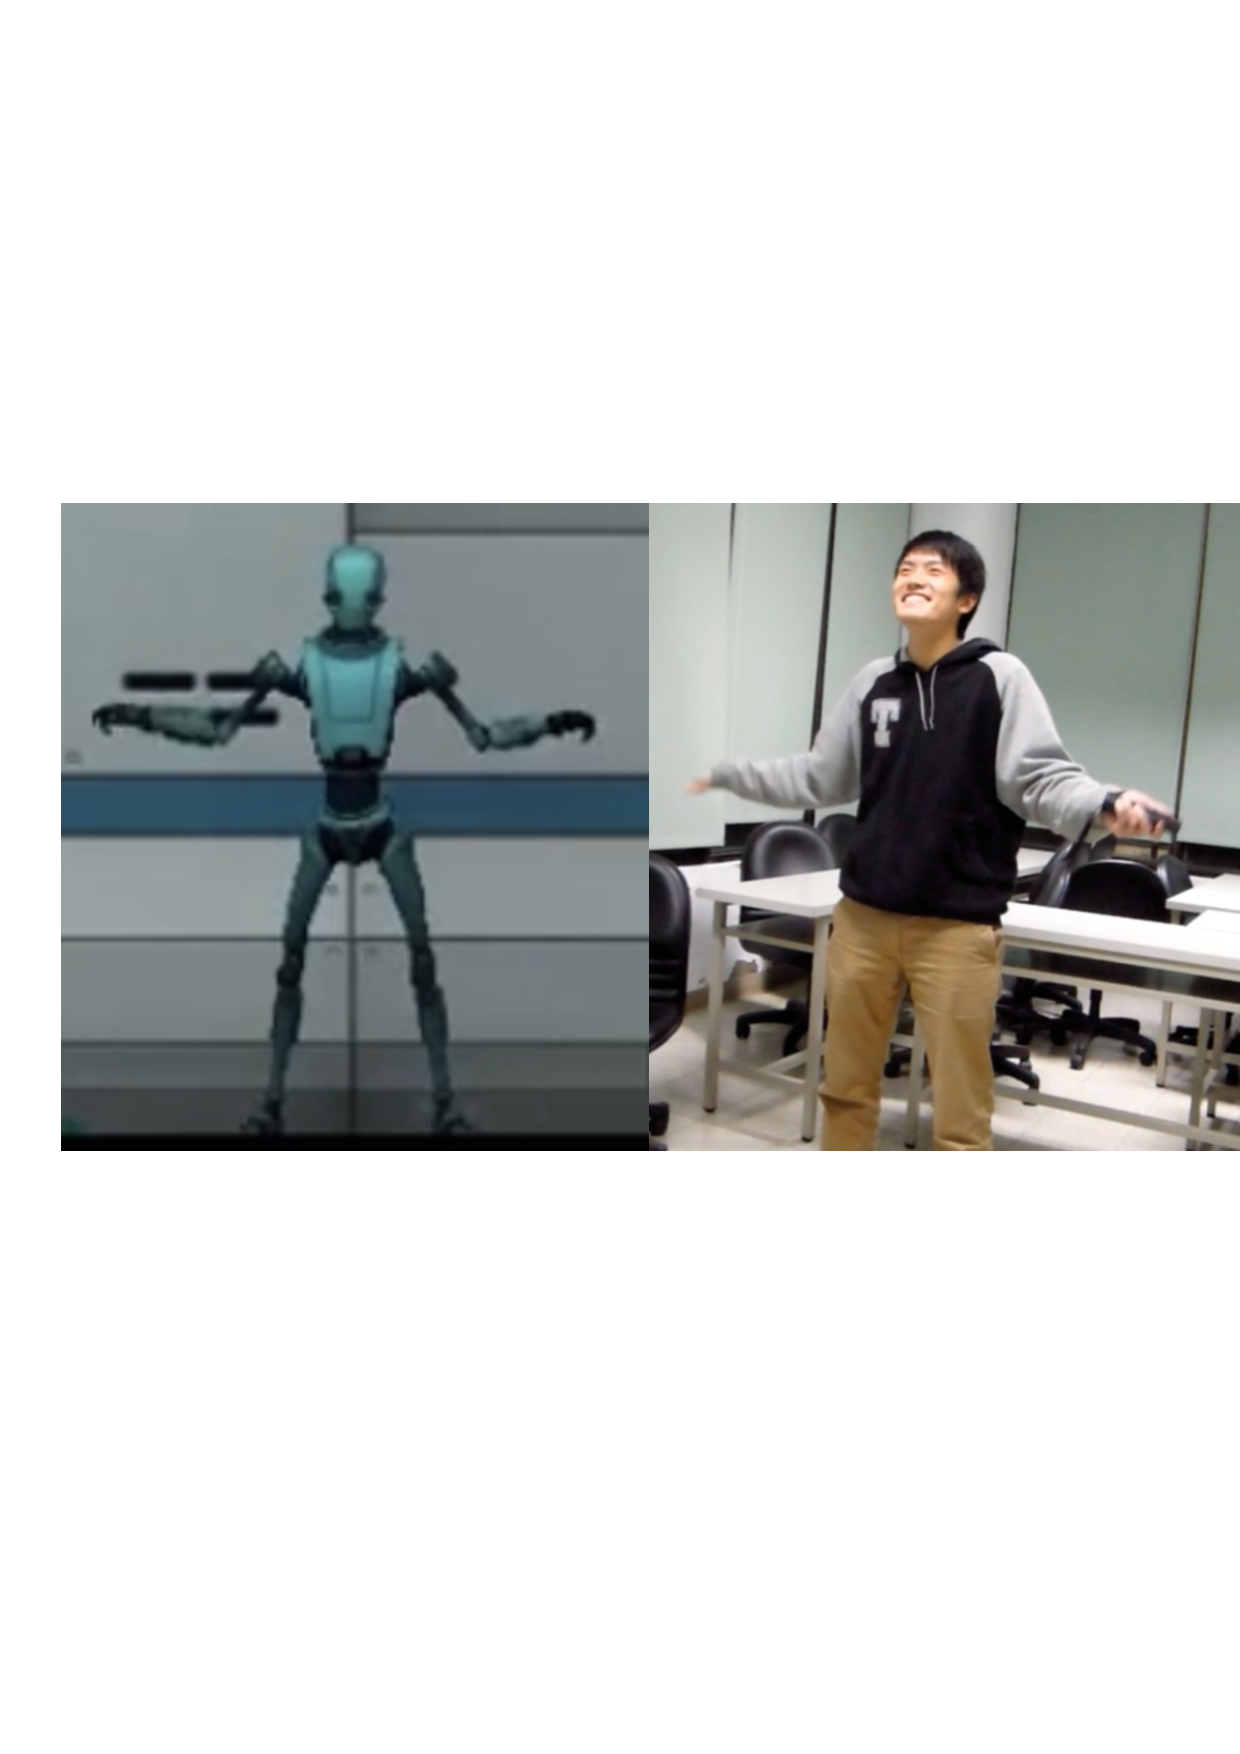
\includegraphics[width=0.9\columnwidth]{Figures/GD_F3.pdf}
\caption{Body movement mapping between player and avatar by Kinect}
\label{fig:GD_F3}
\end{figure}


\begin{figure}[!h]
\centering
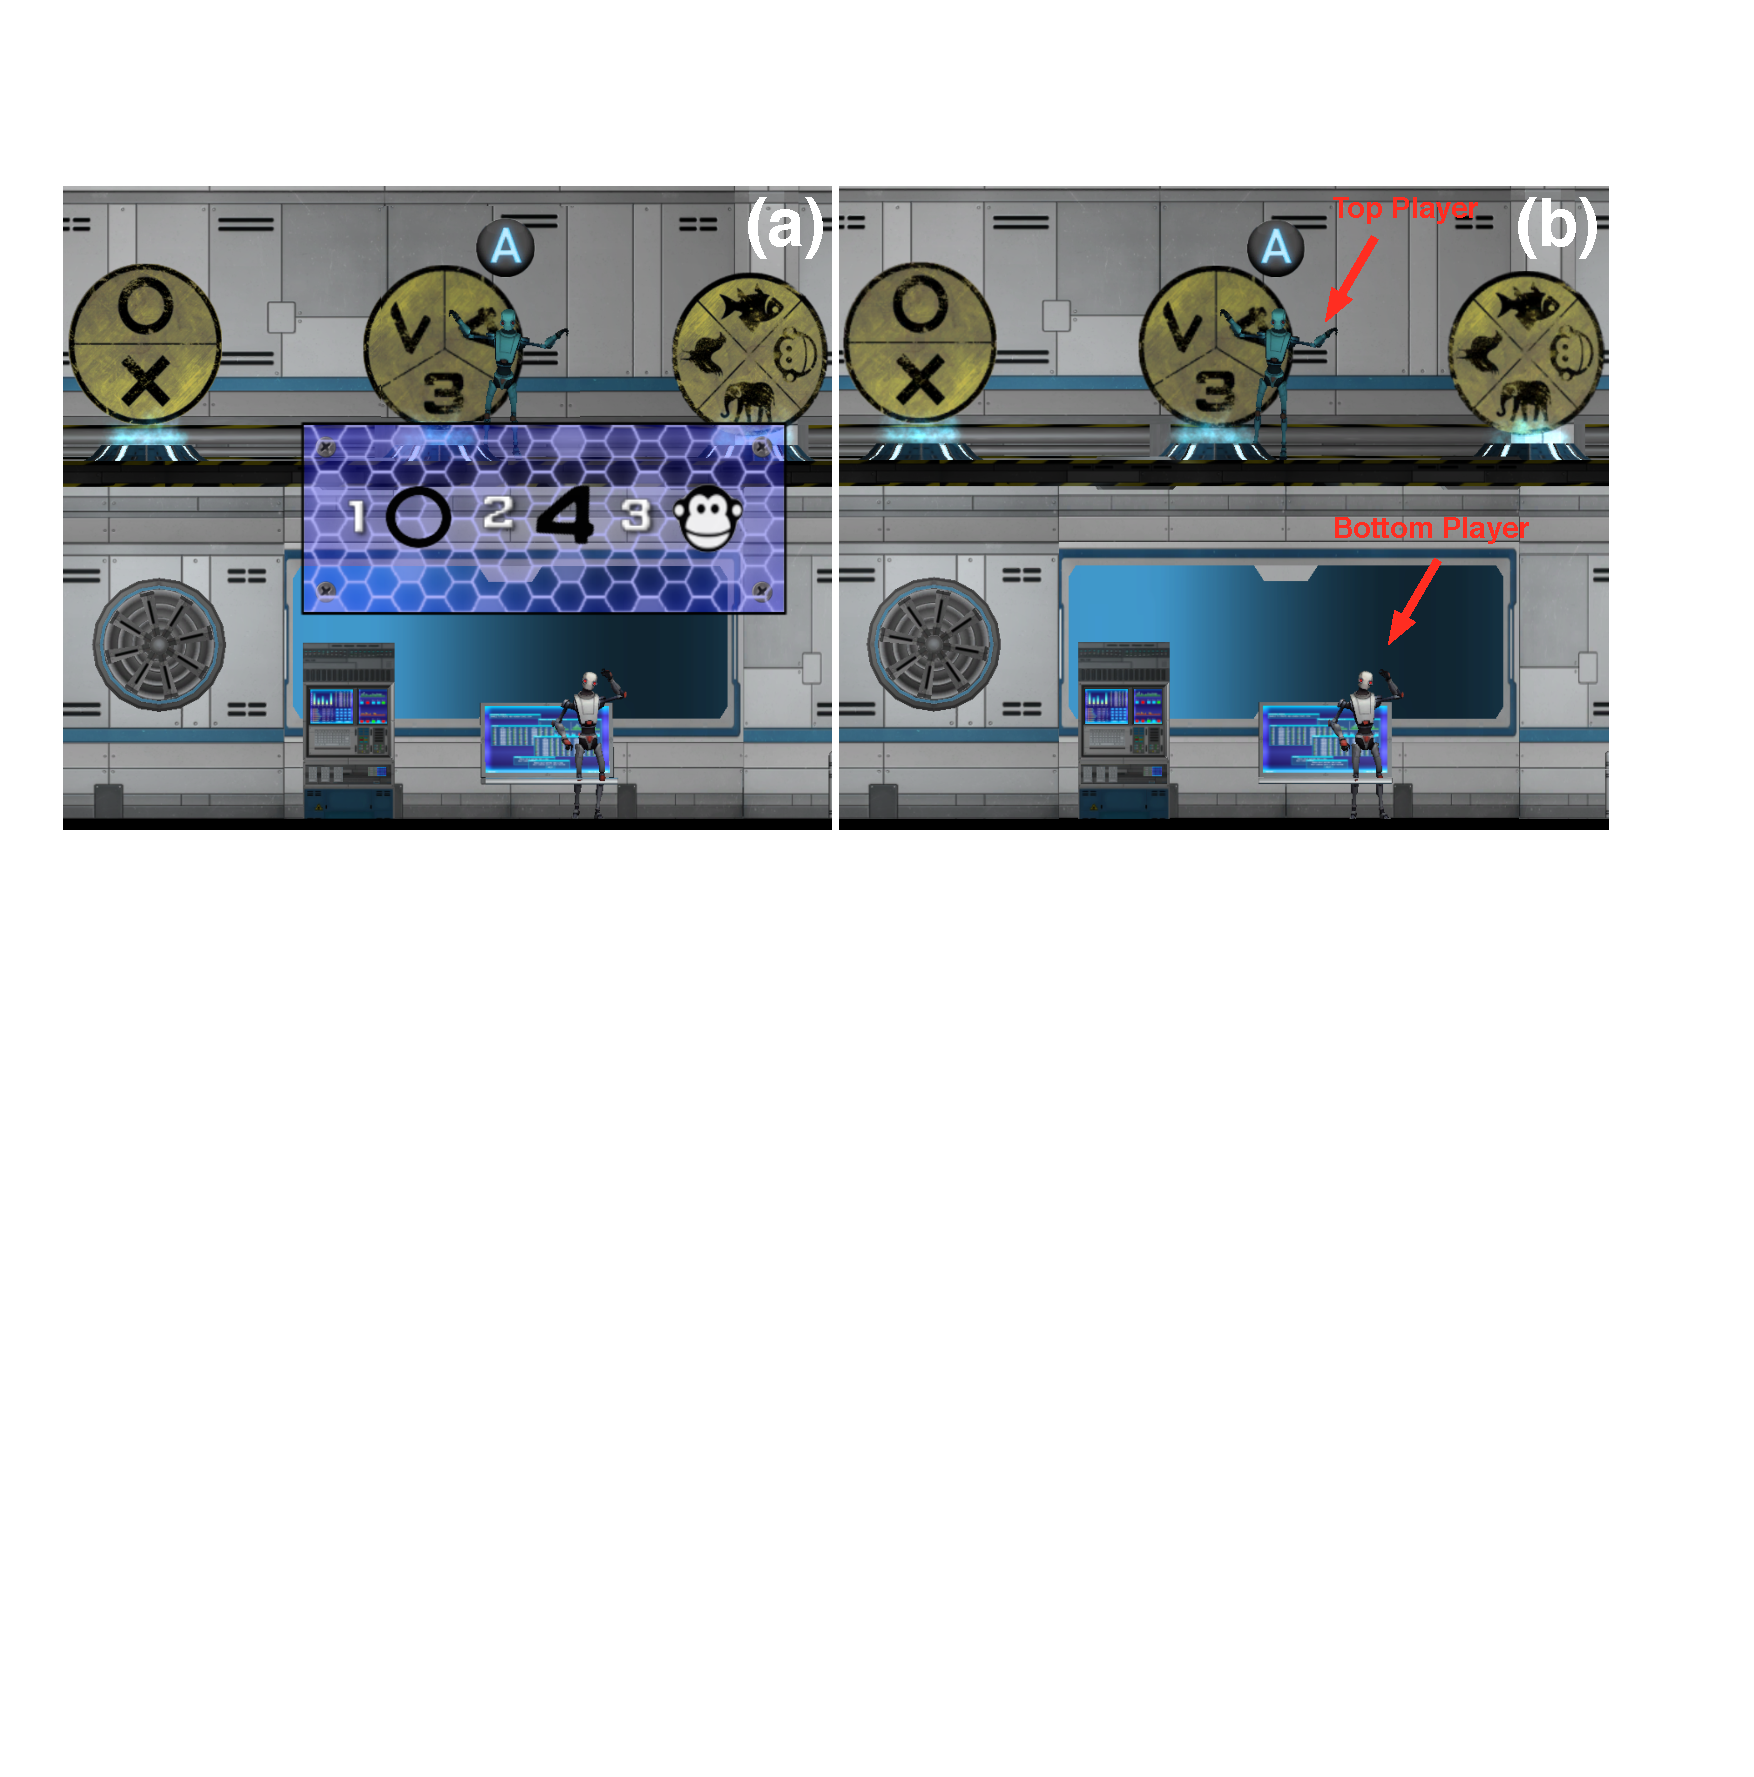
\includegraphics[width=1.0\columnwidth]{Figures/GD_F2.pdf}
\caption{The asymmetric puzzle game design in one of Mute Robot's stages. (a) Bottom player's view, (b) Top player's view}
\label{fig:GD_F2}
\end{figure}


\subsection{Game Level Design}

% To test the limitation of body language in cooperative game, we designed three puzzles with incremental difficulty. Every message for player to transmit is getting more and more complex.

To encourage players to use body language, we have designed an asymmetric puzzle system, with only one player receiving puzzle hints. The player will use body language to guide the other player to solve the puzzle. Taking one of our game stage as an example (see Figure~\ref{fig:GD_F2}), there is a locked door on the right side which obstructs both players' route to the next stage. The top player can't see the puzzle-solving hints but can turn the wheel to match the puzzle answer, which consequently opens the locked door. The only way to pass the stage is for the bottom player to convey the puzzle-solving messages to the other player with body language.

In order to test the limitation of using body language in cooperative game, we designed three puzzles with incremental difficulty, which means that the message player needed to transmit will have higher complexity than the previous one. Next we introduce each game level respectively.

% In the first level, we are testing sequence message to transmit which is a classic cooperative game puzzle. One player has to express the secret sequence to another player, so that he can press the apparatus buttons in correct sequence, then open the door and route to next puzzle.

In the first level, we test sequence messages whether to be transmitted or not. This is a classic puzzle in cooperative game. One player has to express the secret sequence to another player so that another player can press the apparatus buttons in correct order. If the order is correct, the door will open and both players can proceed to the next level.

% In the second level, there are three apparatus wheel to turn to the correct pattern. The symbols on the first wheel are two state of boolean value (circle and cross), and the second wheel’s symbols are numbers (3,4,7), the symbols on the last wheel are animals(fish, chicken, monkey and elephant).

In the second level, there are three apparatus wheels which need to be turned to match the correct pattern. Symbols on the first wheel are boolean value (circle and cross). The second wheel's symbols are numbers (3, 4, 7), and the last wheel's symbols are animals (fish, chicken, monkey and elephant).

% In the last level, we want to test more complex concept like emotion, so we randomly give an emotion word for player to transmit (angry, happy or tired) ,and the player on the other side needs to guess the emotion and spell it correctly.

In the final level, we want to test the concept with higher complexity, such as emotion. So we randomly provide an emotion word (angry, happy or tired) for one player and he needs to transmit to another player. The level can be passed only if another player guesses the emotion and spells it correctly.




